\documentclass{webofc}
\usepackage[varg]{txfonts}   % Web of Conferences font
\begin{document}
\title{System Performance and Cost Modelling in LHC computing}
\author{\firstname{Catherine} \lastname{Biscarat}\inst{1} \and
        \firstname{Tommaso} \lastname{Boccali}\inst{2} \and
        \firstname{Daniele} \lastname{Bonacorsi}\inst{3} \and
        \firstname{Concezio} \lastname{Bozzi}\inst{4,5}\fnsep \and
        \firstname{Raul} \lastname{Cardoso Lopes}\inst{6} \and
        \firstname{Davide} \lastname{Costanzo}\inst{7} \and
        \firstname{Dirk} \lastname{Duellmann}\inst{4} \and
        \firstname{Johannes} \lastname{Elmsheuser}\inst{8} \and
        \firstname{Eric} \lastname{Fede}\inst{9} \and
        \firstname{José} \lastname{Flix Molina}\inst{10} \and
        \firstname{Alessandra} \lastname{Forti}\inst{11} \and
        \firstname{Martin} \lastname{Gasthuber}\inst{12} \and
        \firstname{Domenico} \lastname{Giordano}\inst{4} \and
        \firstname{Costin} \lastname{Grigoras}\inst{4} \and
        \firstname{Jan} \lastname{Iven}\inst{4} \and
        \firstname{Michel} \lastname{Jouvin}\inst{13} \and
        \firstname{Yves} \lastname{Kemp}\inst{12} \and
        \firstname{David} \lastname{Lange}\inst{14} \and
        \firstname{Helge} \lastname{Meinhard}\inst{4} \and
        \firstname{Michele} \lastname{Michelotto}\inst{15} \and
        \firstname{Gareth Douglas} \lastname{Roy}\inst{16} \and
        \firstname{Andrew} \lastname{Sansum}\inst{17} \and
        \firstname{Andrea} \lastname{Sartirana}\inst{18} \and
        \firstname{Markus} \lastname{Schulz}\inst{4} \and
        \firstname{Andrea} \lastname{Sciab\`a}\inst{4} \and
        \firstname{Oxana} \lastname{Smirnova}\inst{19} \and
        \firstname{Graeme} \lastname{Stewart}\inst{4} \and
        \firstname{Andrea} \lastname{Valassi}\inst{4} \and
        \firstname{Renaud} \lastname{Vernet}\inst{20} \and
        \firstname{Torre} \lastname{Wenaus}\inst{8} \and
        \firstname{Frank} \lastname{Wuerthwein}\inst{21}
}

\institute{LPSC Grenoble, IN2P3/CNRS\and
           INFN Sezione di Pisa\and
           University of Bologna \and
           CERN \and
           INFN Sezione di Ferrara \and
           Brunel University \and
           University of Sheffield \and
           Brookhaven National Laboratory \and
           CNRS/IN2P3/LAPP \and
           Centro de Investigaciones Energ\'eticas Medioambientales y Tecnol\'ogicas \and
           University of Manchester \and
           Deutsches Elektronen-Synchrotron \and
           Université Paris-Saclay \and
           Princeton University \and
           Universit\`a e INFN, Padova \and
           University of Glasgow \and
           STFC \and
           Centre National de la Recherche Scientifique \and
           Lund University \and
           Centre de Calcul IN2P3 \and
           Univ. of California San Diego
          }

\abstract{The increase in the scale of LHC computing expected for Run
  3 and even more so for Run 4 (HL-LHC) over the next ten years will
  certainly require radical changes to the computing models and the
  data processing of the LHC experiments. Translating the requirements
  of the physics programmes into computing resource needs is a
  complicated process and subject to significant uncertainties. For
  this reason, WLCG has established a working group to develop
  methodologies and tools intended to characterize the LHC workloads,
  better understand their interaction with the computing
  infrastructure, calculate their cost in terms of resources and
  expenditure and assist experiments, sites and the WLCG project in
  the evaluation of their future choices.  This working group started
  in November 2017 and has about 30 active participants representing
  experiments and sites. In this contribution we expose the
  activities, the results achieved and the future directions.}

\maketitle

%Sciaba
\section{Introduction}

Explain motivations, give current extrapolations to the HL-LHC scale.

Describe history of WG, goals, participation, areas of work.

$\leq 1$ page.


%Markus
\section{Workload characterisation and metrics}
\begin{figure}[h]
  \centering
  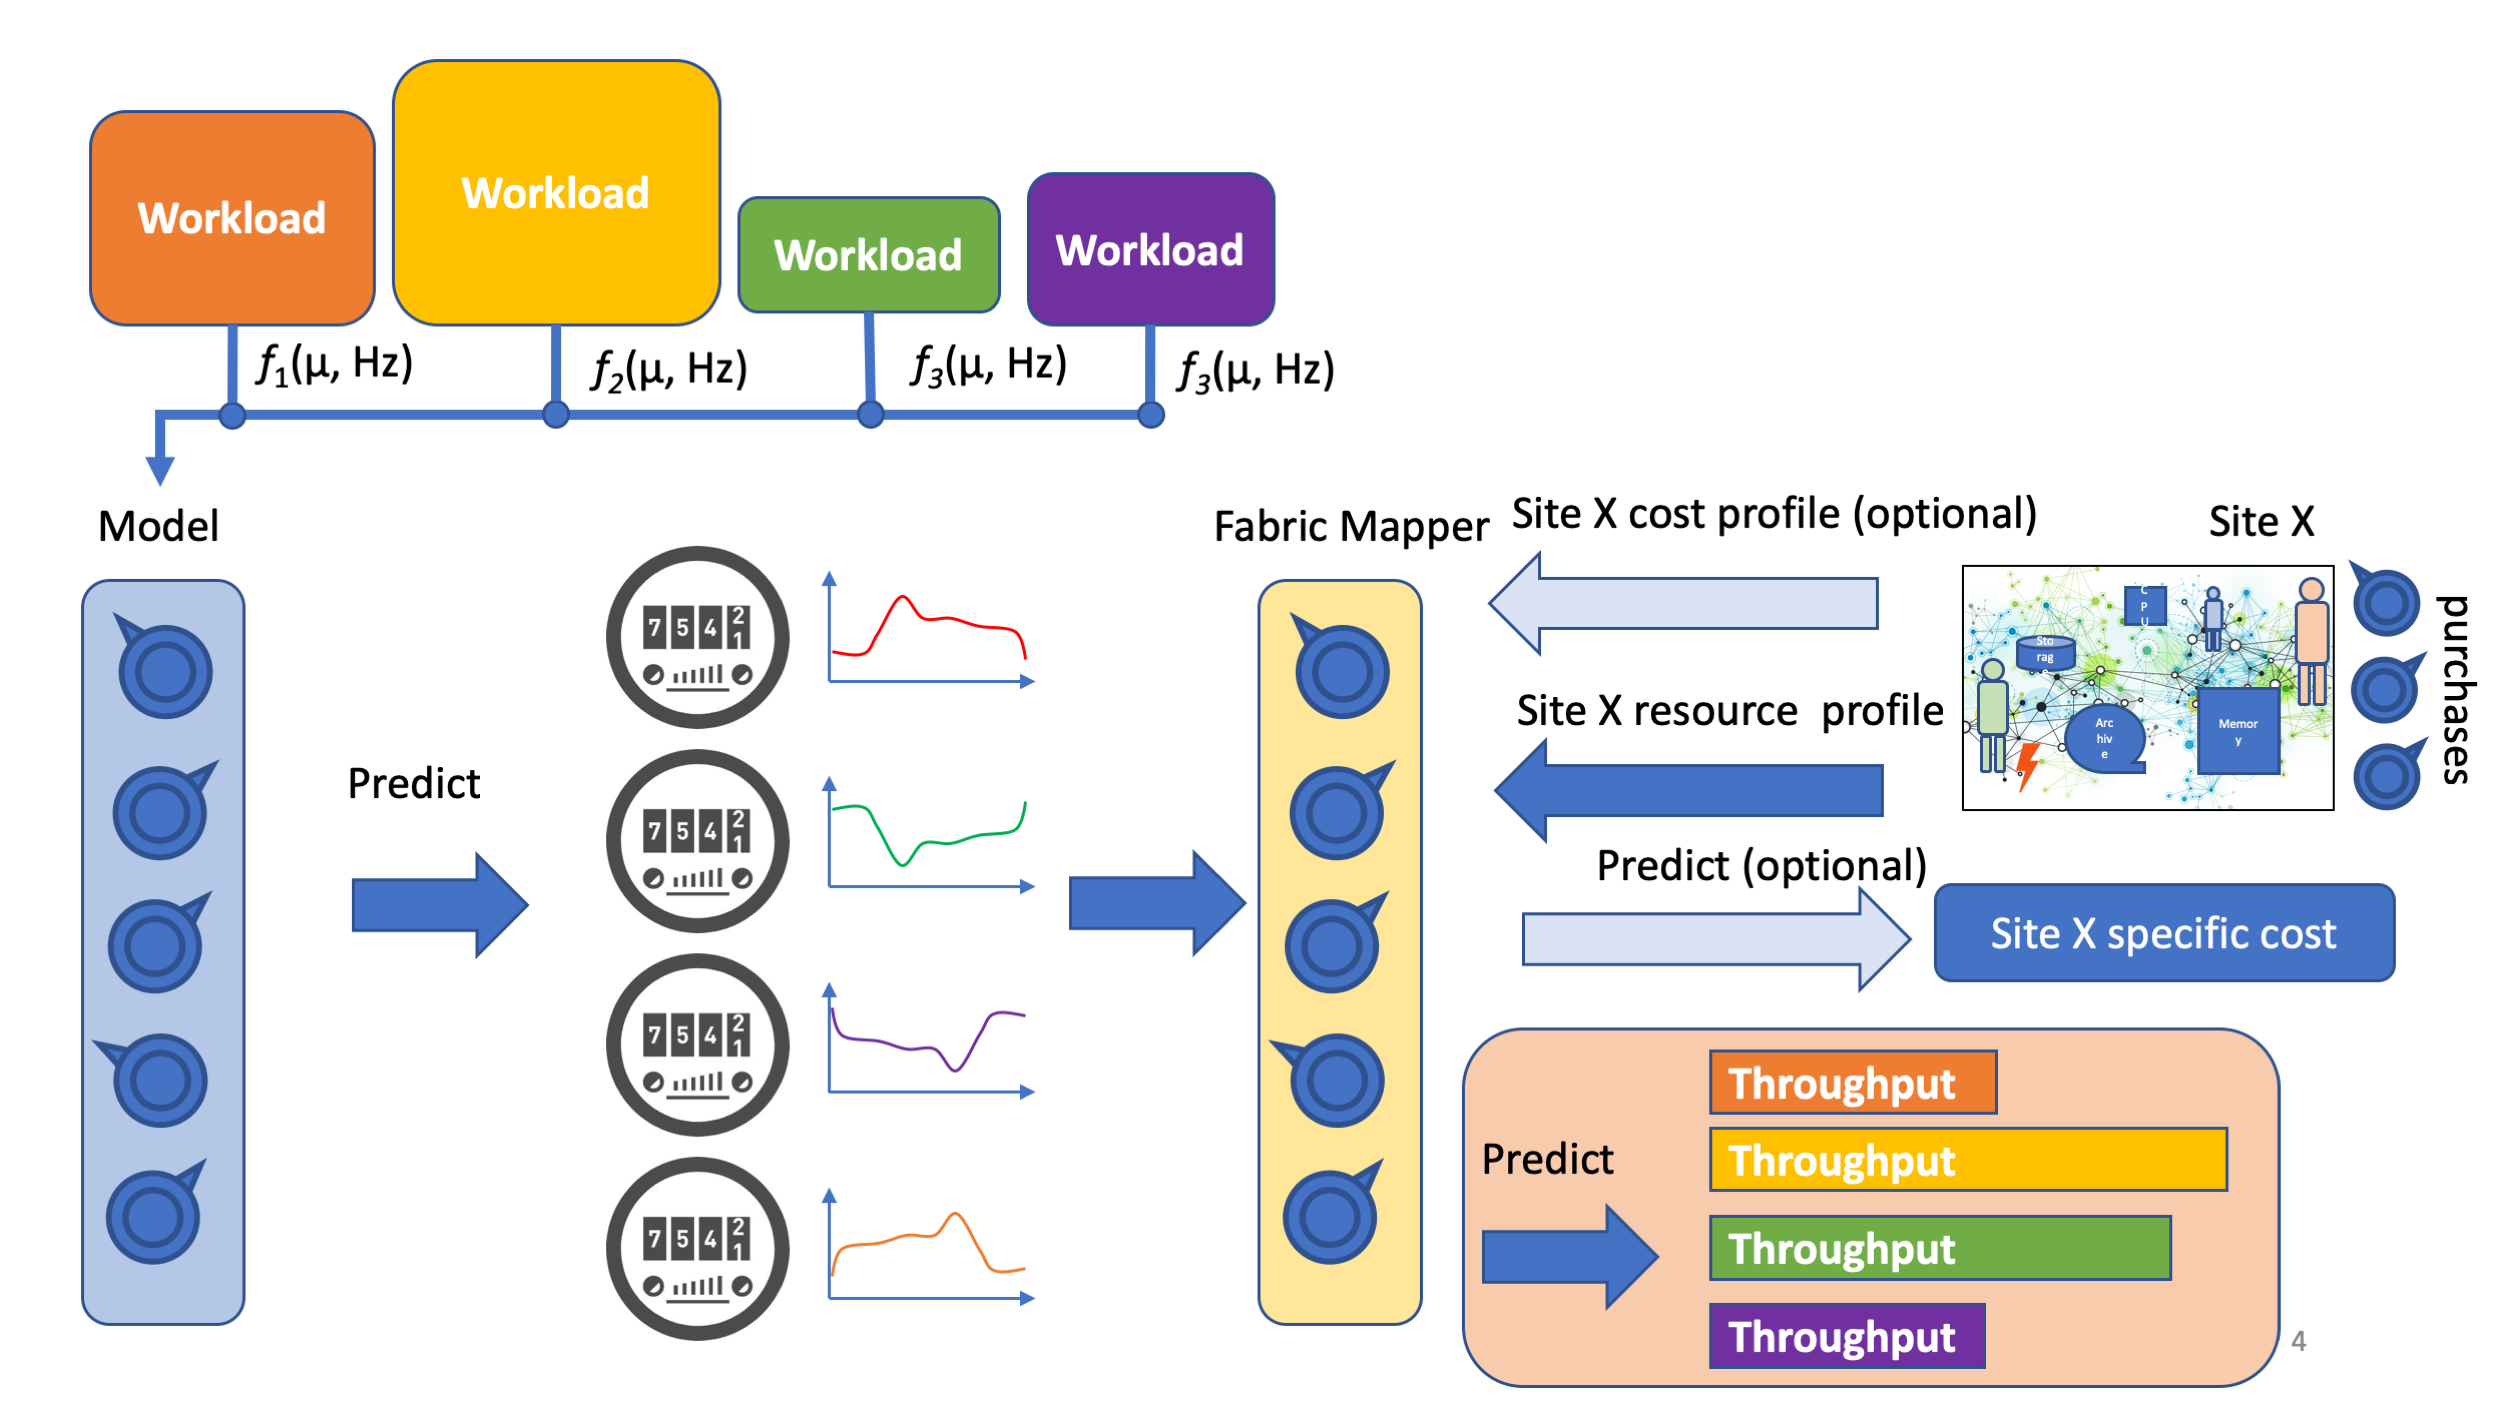
\includegraphics[height=4cm]{CHEP-Model-2.png}
  \hfill
  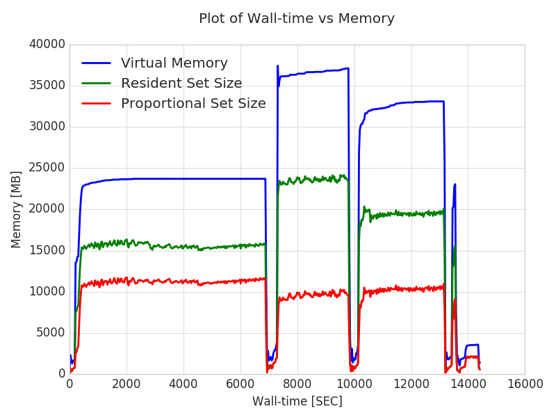
\includegraphics[height=4cm]{prmon.png}
  \caption{{\em (left)} Workload resource requirements depend on the
    pileup and the trigger rate. The model predicts the demands on the
    different resources. The Fabric Mapper abstracts the
    characteristics of a fabric and produces estimates for
    throughputs. Optional sites can add their local cost structure to
    the model. {\em (right)} Memory consumption over the execution of
    an ATLAS Digi-Reco job from PrMon; the different processing steps
    are clearly visible. The periods with very low memory consumption
    are due to the merging of intermediate files}
  \label{fig:mapping}
\end{figure}

To model the behaviour of the workloads of the LHC experiments it is
essential to understand how the different capabilities that a site
provides impact their throughput. To limit the complexity of a
performance model, it is desirable to minimise the number of
performance characteristics; this requires to find a set of
``orthogonal'' metrics to which the throughput is sensitive. This
knowledge can then be used by software developers to avoid bottlenecks
by balancing resource usage, and by site managers to optimise their
expenditure. The balance between the amount of memory per core, the
disk performance and the memory speed and latency can be optimised on
the basis of the characterisation of the relevant
workloads. Figure~\ref{fig:mapping} illustrates this relationship.

Finding such a metric set if far from trivial, given the complexity of
workloads and their production environments. We started from a
representative collection of reference workloads for each experiment.
Then, we listed several metrics, grouped in various categories (CPU,
I/O, memory, storage, swap and network) and assessed their
relevance. Finally we focused on those that can be measured without
significant interference with the running workload on nodes. A tool,
PrMon \cite{prmon}, originally developed by ATLAS, has been
generalised and allows to measure a large set of parameters, using
information from the operating system. Figure~\ref{fig:mapping} shows,
as an example, measurements of the memory usage during the execution
of a workload that performs digitisation with pile-up data and
reconstruction for Monte Carlo events.  PrMon allows to estimate which
capabilities of a system limit the throughput and how efficiently
multi-process and multi-threaded applications use their allocated
cores. To study the dependencies on latency, bandwidth and memory
restrictions, another tool has been developed that runs workloads
repeatedly with increasingly restricted bandwidth, memory and
increased latency, measuring the throughput for each configuration.

Another tool, Trident~\cite{trident}, was developed to provide a
convenient access to the information contained in CPU hardware
counters.  These counters provide information on the level of
parallelism exploited by a workload, memory access, cache utilisation
and vector capabilities, etc.~in an abstract and CPU-model dependent
way.  This gives the developer an estimate on how much improvement is
at best possible in exploiting the available resources and
quantitatively understand the limiting factors. The site managers can
use the insights gained from Trident in decisions concerning
trade-offs between different capabilities, like memory speed vs. size
or system disk speed and network.

\subsection{Next steps}
While the time series measured by PrMon give valuable insights, they
cannot be directly used as input for modelling the behaviour of the
workloads. Work on this process has started to parametrise metric time
series, as processing can be described as sequence of steps, each one
looping over events. During each of these steps the resource usage can
be described by a small number of parameters and the number of
processed events. This, in combination with the dependencies on
latency, bandwidth and memory, will allow to predict the throughput of
the current workloads under different conditions.

For the resource modelling under future running conditions the
dependency on the average pile-up has to integrated into the
model. For data size and simulation time, the dependency is at most
linear. For reconstruction, an extrapolation to HL-LHC levels is
currently very uncertain and it would be exponential with the current
algorithms. ATLAS plans to address this issue by introducing closely
spaced tracking layers, to provide precise starting vectors, while CMS
will take advantage of a very high time resolution to distinguish
between hits from different collisions.


%Sartirana
\section{Resource estimation $\leq 1$ page.}

\subsection{Motivations}

In order to sensibly plan their activity and estimate their costs,
experiments need to translate the requirements of their physics
programs into computing resources needs. They thus need a modeling
tool that takes as input the details of the physics activity
%- such as the amount of data from the detector, the fraction of MC
%events needed, the number of events to be analyzed, etc. - 
and the features of the computing model 
%- e.g. the event size, the
%way data is replicated and distributed, the software efficiency, etc -
and outputs the amount and characteristics of the computing resources
required.

Currently, all LHC experiments have their own tools for this task,
often some complex spreadsheets. Our purpose is to provide a common
framework that could standardize, generalize and possibly improve what
each experiment do, in its own specific way, today. This framework
should be as generic and customable as possible, it should define a
schema for the parameters that describe the expected activity and the
characteristics of the computing model, and provide some standard
calculations on these parameters.  Besides providing the experiment
with a standardized way to compute their needs, such framework will
allow us to easily play with different computing model scenarios and
explore potential gains.

\subsection{Current Status}

A first version of the framework \cite{ourresmodel} was obtained by
forking, refactoring and slightly generalizing some python code
\cite{cmsresmodel} used by CMS to estimate HL-LHC requirements.
It is a set of modules and scripts that reads some json inputs
files and produces plots and tables with the required storage and CPU
resources. Inputs are loaded hierarchically so that we can easily
overwrite a generic set of definitions with different special
scenarios. This is handled by the classes and functions defined in the
{\it ResourceModel} module. Parameters include:
\begin{itemize}
\item LHC parameters: trigger rates, live fractions, shutdown years, etc.
\item Computing model: event sizes and processing times, software improvement factors, etc.
\item Storage model: numbers of versions, replicas, etc.
\item Infrastructure: capacity model, T1 disk and tape, etc.
\end{itemize}
The framework computes the number of data and montecarlo events
per year ({\it EventModel} module) using the LHC parameters and some
physics information like the required montecarlo/data ratio. The
functions defined in {\it CPUModel} and {\it StorageModel} modules,
then, translate the number of events into CPU and Storage requirements
for the different activities (reconstruction, montecarlo, analysis).
The module {\it ModelOut} defines functions to create plots and tables.

\subsection{Future Work}

This first version of the framework elicited strong interest from
other LHC experiments ad has been agreed as a common basis for future
development. Generalizing it to all LHC experiments will require
rewriting some of the most CMS-specific parts and making the
parameters schema more flexible.

Besides the inclusion of all LHC experiments, other lines of
development have been proposed.  For example, the model should be
allowed to have generic time granularity (it currently only deals with
yearly data) and should include an estimation of network resources.



%Renaud
\section{Site cost estimation}
%Explain the importance of a common method to estimate the costs for sites
%given the resource needs of the experiments.
%Describe Renaud's model and future perspectives for this area.

$\leq 1$ page.

The IT resources deployed in the data centres contributing to WLCG are an important source of expense for funding agencies.
With the expected amount of data to be recorded at HL-LHC, it is highly desirable for WLCG to estimate the
amount of IT resources that will be available for data processing in sites over time.
Simple projections from the current trends in the IT market, assuming a constant budget in sites over time, indicate that
the available amount of resources across the WLCG will not be sufficient at all to process the HL-LHC data (reference?).
Therefore, it becomes clear that, unless technology revolutions happen in the meantime,
LHC experiments will need to make a different usage of IT resources that sites will deploy.

The purpose of site cost estimations is to understand and measure, at a global scale,
what the data centres typical expenses are, and predict what they may be in years from now.
These results will help experiments plan new computing strategies that
will improve the cost-effectiveness of their resource usage.







%Markus
\section{Areas of improvement}
Since the start of the LHC the community constantly improved the
throughput of the main workflows; however, studies conducted by the
Understanding Performance team and this working group found several
areas in which potential improvements could be
achieved~\cite{improvements}.

\subsection{Compiler and software improvements}
WLCG sites provide a variety of CPU models and HEP code is usually
built to run on the oldest available architectures. This, and
advancements in compilers motivated further studies.

Studies on GEANT simulation, reconstruction and NLO generator code
show gains by compiler and link-based optimisations to be around
20-25\%, including compilation for individual target CPUs, the use of
Intel’s commercial compiler and the use of feedback-directed
optimisation (AutoFDO from Google and Intel). Compiler-based
vectorisation of current production code showed none or minimal
improvements. Reducing the overhead of shared libraries by building
large libraries resulted in large gains on older architectures (e.g.,
a 10\% on Ivy Bridge for ATLAS simulation). It has to be noted that
the use of feedback-directed optimisation requires that the objects
are build statically, which is not always trivial.

From code profiling and a detailed analysis of the dynamic use of
memory allocation, it is known that the current code spends up to 25\%
of the time on memory/object management, due to the frequent creation
and destruction of small objects~\cite{fomtools}. A 60-90\% of
allocations exists for less than $100\mu$s and are smaller than 64
bytes.  By using better strategies for object management, such as
object pools and static vectors, this could be reduced to less than
10\% with relatively minor code refactorisation. At the same time the
data structure layout can be improved for more efficient utilisation
of caches and improved memory access.

The current HEP code executes on modern cores only $0.8-1.5$
instructions per cycle. With the large vector registers provided by
current CPUs the theoretical limit is above 20 IPC for fully
vectorised code, and tuned complex code for HPC systems can reach
about 4 IPC, which can be seen as an upper limit for our code
base. Approaching this limit requires at least a change of the used
data structures and a re-implementation or factorisation of our
algorithms, and therefore it should be taken into consideration when
designing new algorithms.

Gains from new algorithms and the impact of new detector components
cannot be treated here. As the development of the cellular automaton
based, HLT track reconstruction code for the ALICE HLT has shown,
large factors O(100) can in some cases be achieved~\cite{rohr}.

\subsection{Storage}
The LHC community has recently agreed to a scenario where managed
storage is consolidated at a few, very large data centres (the ``data
lake'') as the most promising to achieve significant cost
savings~\cite{cwp}.

For what concerns operational effort, the 2015 WLCG site
survey~\cite{survey} showed that on average Tier-1 sites require 2.5
FTEs for operating storage and Tier-2 sites 0.75 FTEs, with a weak
dependence on the amount of storage. By concentrating managed storage
at a few sites and using only disk caches at
most sites, one can estimate a decrease of the overall number of FTE
for storage operations from around 100 to around 60.

An $80\%$ of used disk in WLCG consists of data formats used for
analysis. Data popularity studies show that on average datasets exist
at $\sim2$ sites and are accessed less than 10 times over a period of
six months, with most accesses in the first month.  We can argue that
data needs to be stored only once in the data lake, and temporarily
cached as needed depending on the client load. Less popular data may
be purged from disk and kept on tape.
Again, analysis of popularity data and storage system monitoring
indicates that only a small fraction of the produced data is active at
any time and a significant fraction (15-20\%) of the data could be
moved to a different storage layer.

Potential savings depend on the retention strategy and the use of
hierarchical storage: what is gained from replacing some amount of
disk with tape is partially offset by the need of more tape drives and
some added complexity in the data migration.

The concentration of data at a few sites requires to limit the impact
of bandwidth limitations and latency on the workload throughput.  We
measured the impact of latency on throughput of various workloads,
showing that for latencies up to 25ms the reduction of throughput can
be limited to 5\% when using Xcache as an additional layer
(table~\ref{tab:latency}).
\begin{table}
  \centering
  \caption{ Summary of cache and latency studies}
  \label{tab:latency}
  \begin{tabular}{llrlr}
    \hline
    Workload & Condition & Latency (ms) & Method & Rel. time \\\hline
    ATLAS Digi-Reco & data on node & 0 & running local & 1.00 \\ 
    ATLAS Digi-Reco & data remote & ~25 & running local & 1.90 \\ 
    ATLAS Digi-Reco & data rem., empty cache & ~25 & Xcache & 1.08 \\ 
    ATLAS Digi-Reco & data rem., pop. cache & ~25 & Xcache & 1.04 \\ 
    ATLAS Derivation & data on node & 0 & running local & 1.00 \\ 
    ATLAS Derivation & data on EOS & < 1 & running local  & 1.02 \\ 
    ATLAS Derivation & data remote & ~25 & running local & 8.30 \\ 
    ATLAS Derivation & data rem., empty cache & ~25 & Xcache & 1.05 \\ 
    ATLAS Derivation & data rem., pop. cache & ~25 & Xcache & 1.03 \\
    CMS Digi-Reco & data local & 0 & added latency & 1.00 \\
    CMS Digi-Reco & data local & 5 & added latency & 1.01 \\
    CMS Digi-Reco & data local & 10 & added latency & 1.04 \\
    CMS Digi-Reco & data local & 20 & added latency & 1.11 \\
    CMS Digi-Reco & data local & 50 & added latency & 1.24 \\\hline
  \end{tabular}
\end{table}

Data redundancy within storage systems is achieved either by
replication (more performant but expensive) or some form of error
encoding (cheaper but less performant). Even larger savings can be
achieved by not using data redundancy at all and re-staging from
tape, or possibly even regenerating, any lost data.
Based on the observed disk failure rate of about 1\% per year in the
CERN EOS system, the relative total cost
of storage and computing at CERN (around 4 HS06/TB), the amount of CPU
time to generate AOD events ($\sim 850$ HS06$\cdot s$) and their size
($\sim 400$ kB), one can naively estimate that the computing cost to
re-generate the AOD data lost to disk failures is $\sim 20\%$ of the
cost to make the storage fully redundant.

In reality, most of the times the lost data would be replicated
elsewhere; one can conservatively estimate that 30-50\% of the disc
costs can be saved. For this approach to be efficient, the process of
recreating individual files has to be automated, which is highly
desirable since other failure modes lead to data loss on a comparable
scale.

\subsection{Gains from improvements in operations}
Scheduling inefficiencies in WLCG can arise from a mismatch between
cores in a system and memory requirements, a mismatch between
requested cores and cores grouped on nodes (the tessellation problem),
batch system or pilot service inefficiencies, delays due to data
staging, I/O waits etc. Site managers have identified some of these
problems and $20-30\%$ of resources may be lost due to them. With
advanced backfilling and more complex job placement strategies,
efficiencies above 90\% can be reached, at the expense of added
complexity in workload management systems. Another source of
scheduling inefficiencies stems from breaking the processing chains
from raw data to data analysis objects into several individual steps
that exchange data via files: especially when parallel processing
threads/processes write individual files, the merging steps create
inefficiencies, as they are single threaded. By using shared writers
these inefficiencies can be reduced. The overall impact is difficult
to measure, but from ATLAS step chain activity logs it can be
estimated to be about 5\%.

Losses due to occasional job failures are unavoidable. Currently most
of the steps can recover from failure with the help of automated retry
mechanisms, but complete jobs are sometimes run up to 20 times before
successful completion. The overall loss in walltime due to job
failures is between 10 and 15\%. Improved procedures to make jobs more
resilient or fail very early can reduce these losses.

Table~\ref{tab:pgain} summarises the different identified potential gains.

\begin{table}
  \centering
  \caption{Estimated potential gains and associate efforts}
  \label{tab:pgain}
  \begin{tabular}{llll}
    \hline
    Change & Effort for sites & Effort for users & Potential gain \\\hline
    Managed storage only at few sites & some on large sites & little & $-40\%$ effort \\
    Reduced data redundancy & some on large sites & some & $-30$-$50\%$ cost \\
    Scheduling and site inefficiencies & some & some & $+10$-$20\%$ CPU  \\
    Reduced job failure rates & little & some - massive & $+5$-$10\%$ CPU \\
    Compiler and build improvements & none &  little - some & $+15$-$20\%$ CPU \\
    Improved memory usage & none & some &  $+10$-$15\%$ CPU \\ 
    Exploiting modern CPU arch. &  none & massive & $+100\%$ CPU \\\hline
  \end{tabular}
\end{table}


%Sciaba
\section{Conclusions}
Conclusions.

$\leq 0.5$ pages.


\begin{thebibliography}{}
\bibitem{RefJ}
% Format for Journal Reference
Journal Author, Journal \textbf{Volume}, page numbers (year)
% Format for books
\bibitem{RefB}
Book Author, \textit{Book title} (Publisher, place, year) page numbers
% etc
\end{thebibliography}


\end{document}

